
\section{Simple distributed image reconstruction}\label{dist}
Show architecture

Different architectures, why don't we do consensus algorithms.

Message Passing Interface (MPI)


Gridding and Devonvolution

We use the recently developed Image Domain Gridder (IDG) 


\subsection{The Image Domain Gridder}\label{distribution:idg}

What the gridding actually does. In theory, just an interpolation. Interpolation kernel like Spheroidal, Kaiser-Bessel functions etc. Generally the most intensive step, because the number of grid cells is generally a lot smaller than the number calibrated Visibilities.

However, here we move from the three dimensional Visibilities to two dimensions. DDE's fall down in the area of the gridder.

So how we do an interpolation 

Veeneboer et al\cite{veenboer2017image} developed the Image Domain Gridder. It uses Subgrids and solves each subgrid seperately.
It is in the image domain, because it can do Radio Interferometer specific corrections efficiently. Furthermore, it leads to a structure which is primed for GPU processing.
We use this algorithm to distribute the gridding.

W-Projection, Spheroidal are convolutions in the Fourier space.

The figure \ref{distribution:idg:system} shows the different parts of the image domain algorithm.

\begin{figure}[h]
	\centering
	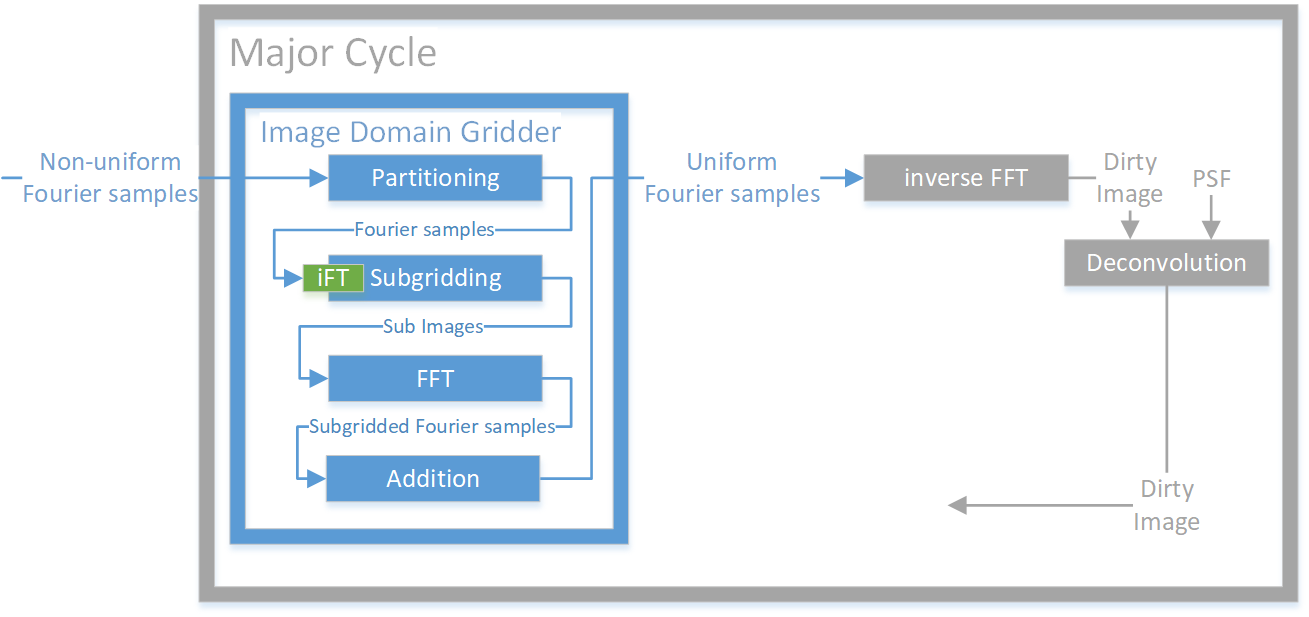
\includegraphics[width=0.80\linewidth]{./chapters/03.distribution/idg/major-minor-idg.png}
	\caption{Image Domain Gridder in the Major Cycle Architecture}
	\label{distribution:idg:system}
\end{figure}

Algorithm
\begin{figure}[h]
	\centering
	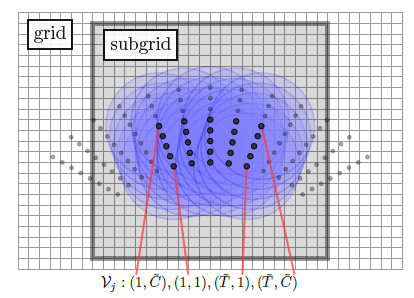
\includegraphics[width=0.40\linewidth]{./chapters/03.distribution/idg/subgrid.png}
	\caption{Subgrid}
	\label{distribution:idg:subgrid}
\end{figure}

\begin{figure}[h]
	\centering
	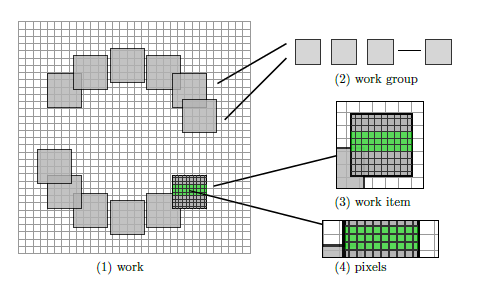
\includegraphics[width=0.40\linewidth]{./chapters/03.distribution/idg/paralellization.png}
	\caption{parallel}
	\label{distribution:idg:parallel}
\end{figure}

\begin{figure}[h]
	\centering
	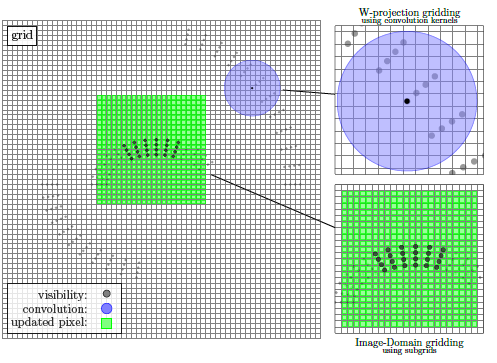
\includegraphics[width=0.40\linewidth]{./chapters/03.distribution/idg/idg0.png}
	\caption{Image Domain Gridder in the Major Cycle Architecture}
	\label{distribution:idg:idg0}
\end{figure}

\subsection{Coordinate Descent deconvolution}

Coordinate Descent Algorithm why

Variants

Implementation
Correlate the dirty image
Find max
How to calculate a

\subsubsection{ElasticNet Regularization}
Why


Formula

\begin{figure}[h]
	\centering
	\begin{subfigure}[b]{0.3\linewidth}
		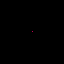
\includegraphics[width=\linewidth]{./chapters/03.distribution/L1.png}
		\caption{Effect of the pure L1 norm ($\lambda$ = 0.1) on a single point source.}
		\label{dist:cd:elastic:L1}
	\end{subfigure}
	\begin{subfigure}[b]{0.3\linewidth}
		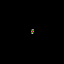
\includegraphics[width=\linewidth]{./chapters/03.distribution/L2.png}
		\caption{Effect of the pure L2 norm ($\lambda$ = 0.1) on a single point source.}
		\label{dist:cd:elastic:L2}
	\end{subfigure}
	
	\caption{Effect of the L1 and L2 Norm separately.}
	\label{dist:cd:elastic}
\end{figure}


Effect

Implementation



May even speed up convergence for correlated pixel values compared to L1 or L2\cite{friedman2010regularization}. But was not investigated in this project

\subsection{Major Cycle convergence}
Putting it all together

We have the Minor Cycle, which is easy to converge.

Coordinate Descent Path optimization \cite{friedman2010regularization}
Danger that CD takes too many pixel into a Major Cycle. Lower bound per iteration, PSF sidelobe
  can still be too low, danger when many psf sidelobes overlap

\subsection{Test on MeerKAT data}

